\documentclass{article}
\usepackage{graphicx} % Required for inserting images
\usepackage{url}
\usepackage{hyperref}
\usepackage{fancyhdr}
\usepackage[mathscr]{euscript}
\usepackage{mathtools}
\usepackage{amsfonts}
\usepackage{amsmath}
\usepackage[margin=1in]{geometry}
\usepackage{pgfplots}
\usepackage{natbib}
\usepackage{mathrsfs}
\pgfplotsset{compat=1.15}

\pagestyle{fancy}
\cfoot{}
\rhead{Probabalistic ML Project Proposal}
\rfoot{\thepage}

\title{Project - Image Generation Models from a Probabilistic Perspective}
\author{Amro Alabsi Aljundi (nmm2uy) | Nate Kimball (tma5gv) | Patrick Soga (zqe3cg)}
\date{April 2024}

\begin{document}


\newcommand{\pt}{p_\theta}
\newcommand{\qp}{q_\phi}
\newcommand{\E}{\mathbb{E}}
\newcommand{\Eqp}{\E_{\qp}}
\newcommand{\Eql}{\E_{\qp(z|x^{(i)})}}
\newcommand{\kl}{D_{KL}}
\newcommand{\loss}{\mathcal{L}(\theta,\phi;x^{(i)})}
\newcommand{\lossA}{\tilde{\mathcal{L}}^A(\theta,\phi;x^{(i)})}
\newcommand{\lossB}{\tilde{\mathcal{L}}^B(\theta,\phi;x^{(i)})}
\newcommand{\bt}{\beta_{t}}
\newcommand{\at}{\alpha_t}
\newcommand{\aht}{\bar{\alpha}_t}
\newcommand{\N}{\mathcal{N}}
\newcommand{\amro}[1]{({\color{blue} amro: #1})}
\DeclarePairedDelimiter{\norm}{\lVert}{\rVert}

\maketitle

\section{Proposal}

Diffusion models have demonstrated impressive image-generation abilities, exceeding those of techniques like generative adversarial networks (GAN) and autoregressive models. 
We will investigate \href{https://en.wikipedia.org/wiki/Diffusion_model}{Diffusion Models} from a probabilistic standpoint. We will begin by explaining the class of \href{https://en.wikipedia.org/wiki/Variational_Bayesian_methods}{Variational Bayesian Methods} and their relationship with diffusion models.
DPMs (diffusion models) can be viewed as a type of \href{https://en.wikipedia.org/wiki/Variational_autoencoder}{variational autoecoder (VAE)}~\citep{Kingma2014, pmlr-v32-rezende14}. 

Specifically, we will first explain the inner workings of variational autoencoders (VAEs) \citep{Kingma2014} for image generation, and then introduce the essential concepts and mathematical background necessary for diffusion models \citep{ho-denoising} as originally defined. Finally, we will connect VAEs with diffusion models from a Bayesian variational perspective, explaining and analyzing work by \cite{kingma-vdm} on variational diffusion models and investigating the improvements on image generation quality that diffusion can provide.

\section{Auto-Encoding Variational Bayes}
Kingma and Welling introduce a stochastic variational inference and learning algorithm for approximating intractable posteriors. With a reparameterization of the variational lower bound, they produce a simpler and more stable lower bound that can be optimized with standard stochastic gradient methods. To do posterior inference on i.i.d. datasets with continuous latent variables per datapoint, they fit an approximate inference model to the intractable posterior using their lower bound estimator. Essentially, they are trying to approximate the distribution of latent variables, underlying lower-dimensional information in the data. They do this by finding an optimizable lower bound on the log-likelihood of the data. In optimizing this lower bound, they learn the parameters for a recognition model, an approximation of the latent posterior, and a generative model, the likelihood of the data given the latent variables. They also propose the Variational Autoencoder architecture for applying their loss function to image generation. \\

\subsection{Problem Scenario}
You have a dataset $\mathcal{D} = \{x^{(i)}\}_{i=1}^n,~ x^{(i)}$ i.i.d., where each datapoint is associated with a continuous latent variable. We assume each datapoint is generated by the following random process:
\begin{enumerate}
    \item a value $z^{(i)}$ is generated according to some prior distribution $p_{\theta^*}(z)$
    \item a value $x^{(i)}$ is generated from some conditional distribution $p_{\theta^*}(x|z)$
\end{enumerate}
We assume that the prior $p_{\theta^*}(z)$ and likelihood $p_{\theta^*}(x|z)$ come from parametric families of distributions of $\pt(z)$ and $\pt(x|z)$, and that their PDFs are differentiable almost everywhere w.r.t. both $\theta$ and z. Commonly, this means assuming our distribution can be represented by a specific neural network. This simplifies our search space. $\theta^*$ and $z^{(i)}$ are unknown to us. \\

We want to find an efficient algorithm that avoids the following obstacles:
\begin{enumerate}
    \item Intractability: The integral of the marginal likelihood $\pt(x) = \int \pt(z)\pt(x|z)dz$ is intractable, and the true posterior density $\pt(z|x) = \pt(x|z)\pt(z)/\pt(x)$ is intractable so the EM algorithm cannot be used. Intractability is common when working with moderately complicated likelihood functions $\pt(x|z)$, e.g. a non linear neural network 
    \item Large dataset: With a large dataset, batch optimization is too costly, and sampling-based solutions, e.g. Monte Carlo EM, are too slow. Minibatch or single datapoint parameter updates are preferable.
\end{enumerate}

The authors propose a solution to the following problems in this scenario:
\begin{enumerate}
    \item $\hat{\theta}$: efficient approximate ML or MAP estimation for the parameters $\theta$.
    \item $\pt(z|x)$: efficient approximate posterior inference of the latent variable $z$ given an observed value $x$ and parameters $\theta$, aka encoding.
    \item $\pt(x)$: efficient approximate marginal inference of the variable $x$ aka synthesis.
\end{enumerate}

\subsection{The Variational Method}
Variational methods allow us to avoid the intractable integral by transforming the statistical inference problem into an optimization problem. We will learn an approximation of the true posterior, which we call a recognition model, denoted by $\qp(z|x)$. We introduce a method for learning the recognition model parameters $\phi$ jointly with the generative model parameters $\theta$. Our goal is to find the best approximation of $\pt(z|x)$, so we start by minimizing the KL-divergence between $\qp(z|x)$. and $\pt(z|x)$.\\
\begin{align}
    \phi^*,\theta^* = \underset{\phi,\theta}{\mathrm{argmin}} ~\kl(\qp(z|x)||\pt(z|x))
\end{align}
We further reduce this term to derive what is known as the \textit{evidence lower bound} (ELBO).
\begin{align}
    \kl(\qp(z|x^{(i)})||\pt(z|x^{(i)})) &= \int_z \qp(z|x^{(i)})\log{\frac{\qp(z|x^{(i)})}{\pt(z|x^{(i)})}}dz \\
    &= \int_z \qp(z|x^{(i)})\log{\qp(z|x^{(i)})}dz - \int_z \qp(z|x)\log{\pt(z|x^{(i)})}dz \\
    &= \E_{\qp(z|x)}[\log (\qp(z|x^{(i)}))] - \mathbb{E}_{\qp(z|x)}[\log (\pt(z|x^{(i)}))] \\
    &= \E_{\qp(z|x)}[\log (\qp(z|x^{(i)}))] - (\E_{\qp(z|x)}[\log (\pt(x^{(i)},z))] - \E_{\qp(z|x)}[\log p(x^{(i)}]) \\
    &= \E_{\qp(z|x)}[\log (\qp(z|x^{(i)}))] - \E_{\qp(z|x)}[\log (\pt(x^{(i)},z))] + \log p(x^{(i)}) \label{eq:elbo}\\
    &= -\text{ELBO} + \log \pt(x^{(i)})\label{eq:likelihood}
\end{align}
The term $\log p(x^{(i)})$ is a constant for a particular data point, so it can be ignored during the optimization process. We can rewrite the evidence lower bound as follows:
\begin{align}
    \text{ELBO} &= -\E_{\qp(z|x)}[\log (\qp(z|x^{(i)}))] + \E_{\qp(z|x)}[\log (\pt(x^{(i)},z))]  \label{eq:elbo1}&\text{from eq. (\ref{eq:elbo})}\\
    &= -\E_{\qp(z|x)}[\log (\qp(z|x^{(i)}))] + \E_{\qp(z|x)}[\log p_{\theta}(z)] + \E_{\qp(z|x)}[\log (\pt(x^{(i)}|z))] \\
    &= -\kl(\qp(z|x^{(i)})||\pt(z)) + \E_{\qp(z|x)}[\log (\pt(x^{(i)}|z))] \label{eq:elbo_simplified}
\end{align}
Using equation \ref{eq:likelihood}, we can show that the evidence lower bound is a lower bound on the marginal log-likelihood of the data $\log \pt(x^{(i)})$:
\begin{align}
    \log \pt(x^{(i)}) &= \text{ELBO} + \kl(\qp(z|x^{(i)})||\pt(z|x^{(i)})) \\
    \log \pt(x^{(i)}) &\geq \text{ELBO}
\end{align}
We can reformulate the original optimization process as:
\begin{align}
\phi^*,\theta^* &= \underset{\phi,\theta}{\mathrm{argmin}} ~\kl(\qp(z|x)||\pt(z|x)) \\ 
&= \underset{\phi,\theta}{\mathrm{argmax}}~\text{ELBO} \\
&= \underset{\phi,\theta}{\mathrm{argmax}} \left[-\kl(\qp(z|x)||\pt(z)) + \E_{\qp(z|x)}[\log (\pt(x^{(i)}|z))]\right]
\end{align}

\subsection{Optimizing the Lower bound}
We will define our likelihood estimator as the evidence lower bound.
\begin{align}
    \log \pt(x^{(i)}) \geq \loss = -\kl(\qp(z|x)||\pt(z)) + \Eqp[\log (\pt(x^{(i)}|z))] \label{eq:likelihood_estimate}
\end{align}
We want to optimize the lower bound w.r.t. both the variational parameters $\phi$ and generative parameters $\theta$. However, this requires sampling $q_\phi(z|x)$ to compute each latent. This process is generally not differentiable, so the gradient w.r.t. $\phi$ is problematic. One way to estimate this gradient is to use a Monte Carlo gradient estimator:
\begin{align}
    \nabla_\phi \E_{q_\phi(z)}[f(z)] = \E_{q_\phi(z)}[f(z)\nabla_{q_\phi(z)}\log \qp(z)] \simeq \frac{1}{L}\sum_{l=1}^Lf(z)\nabla_{q_\phi(z^{(l)})}\log \qp(z^{(l)}) \\ \notag \text{~where~} z^{(l)} \sim \qp(z|x^{(i)}) \label{eq:MonteCarlo}
\end{align}
This gradient estimator exhibits very high variance and is impractical in many cases, because $\qp$ can be an arbitrarily complicated distribution that is hard to sample. Since we sample from $\qp(z|x^{(i)})$, the gradients of the MC estimate term in the loss can only be back-propagated up to the sampled latent variable $z^{(l)}$. The gradient of $z^{(l)}$ w.r.t. $\phi$ can not be computed. Thus, only the KL divergence term can optimize $\phi$ leading to an unstable suboptimal learning process.

\subsubsection{The SGVB estimator and AEVB algorithm}\label{reparam}
To resolve this issue, we employ the \textit{reparameterization trick}, which allows us to backpropagate loss w.r.t. $\phi$ through the decoder and encoder by treating $q_\phi$ as a differentiable deterministic function by isolating randomness to an auxiliary variable. Under certain mild conditions for $\qp(z|x)$, we can reparameterize each latent $\Tilde{z} \sim \qp(z|x)$ using a differentiable transformation $g_\phi(\epsilon,x)$ of an auxiliary noise variable $\epsilon$:
\begin{align}
    \Tilde{z} = g_\phi(\epsilon,x)~\text{with}~\epsilon \sim p(\epsilon)
\end{align}
\begin{figure}[b]
    \centering
    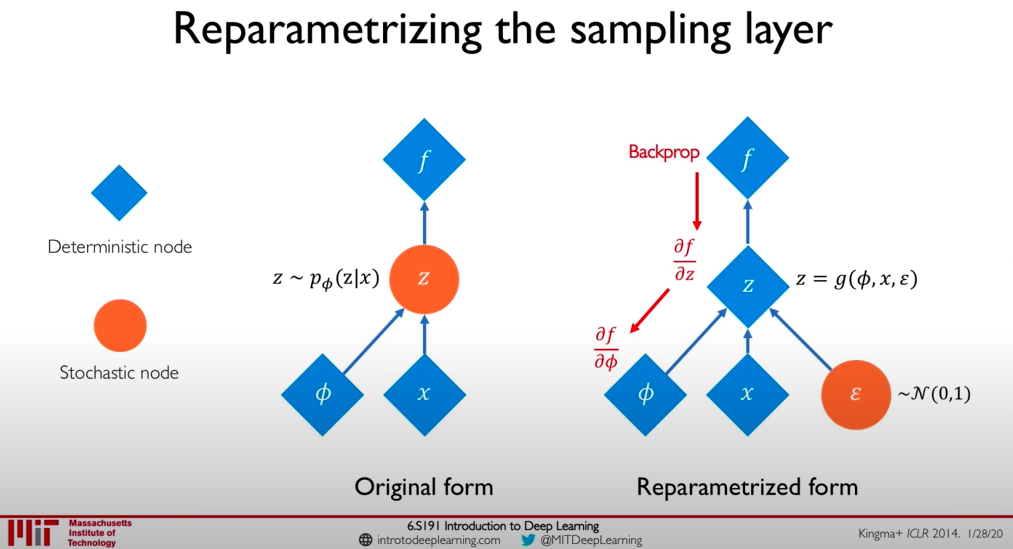
\includegraphics[scale=.25]{reparameterization_trick.png}
    \caption{Reparameterization Trick Visualization}
    \label{fig:reparam}
\end{figure}
We can now rewrite samples from $\qp(z|x)$ in terms of $g_\phi$ and form Monte Carlo estimates of expectations as follows:
\begin{align}
    \Eql[f(z)] = \E_{p(\epsilon)}[f(g_\phi(\epsilon,x^{(i)}))] \simeq \frac{1}{L}\sum^L_{l=1}f(g_\phi(\epsilon^{(l)},x^{(i)})) \notag \\
    \text{where}~\epsilon^{(l)} \sim p(\epsilon)
\end{align}
By applying this technique to the variational lower bound eq. (\ref{eq:elbo1}), we get our generic Stochastic Gradient Variational Bayes (SGVB) estimator $\lossA\simeq\loss$:
\begin{align}
    \lossA = \frac{1}{L}\sum_{l=1}^L\log\pt(x^{(i)},z^{(i,l)}) - \log\qp(z^{(i,l)}|x^{(i)}) \notag \\\text{~~where~~} z^{(i,l)} = g_\phi(\epsilon^{(i,l)},x^{(i)}) \text{~~and~~} \epsilon^{(l)}\sim p(\epsilon)
\end{align}
Often, the KL-Divergence $\kl(\qp(z|x^{(i)})||\pt(z))$ from eq. (\ref{eq:elbo_simplified}) can be integrated analytically such that only the expected reconstruction error $\Eqp[\log (\pt(x^{(i)}|z))]$ requires estimation by sampling. The KL-divergence term can then be interpreted as regularizing $\phi$, encouraging the approximate posterior to be close to the prior $\pt(z)$. This leads to a new lower-variance SGVB estimator $\lossB\simeq\loss$:
\begin{align}
    \lossB = -\kl(\qp(z|x^{(i)})||\pt(z)) + \frac{1}{L}\sum_{l=1}^L\log\pt(x^{(i)}|z^{(i,l)}) 
    \notag \\
    \text{where~~} z^{(i,l)} = g_\phi(\epsilon^{(i,l)},x^{(i)}) \text{~~and~~} \epsilon^{(l)}\sim p(\epsilon)
\end{align}

\subsection{Example: Variational Auto-Encoder}
For VAEs, we will use a neural network for the probabilistic encoder $\qp(z|x)$. Let $\pt(x|z)$ be a multivariate Gaussian (for continuous data) or Bernoulli (for binary data) distribution whose parameters are computed from $z$ with an MLP. We assume the true but intractable posterior $\pt(z|x)$ takes on an approximate Gaussian form with approximately diagonal covariance:
\begin{align}
    \log\qp(z|x^{(i)}) = \log\N(z;\mu^{(i)},\sigma^{2(i)}\mathbf{I})
\end{align}
where the mean and s.d. of the approximate posterior, $\mu^{(i)}$
and $\sigma^{(i)}$, are outputs of the encoding MLP. \\
We sample from the posterior $z^{(i,l)}\sim\qp(z|x^{(i)})$ using $z^{(i,l)} = g_\phi(x^{(i)}) = \mu^{(i)} + \sigma^{(i)} \odot \epsilon^{(l)}$ where $\odot$ stands for element-wise multiplication. We assume our prior over the latent space is the standard normal distribution: $\pt(z)=\N(0,\mathbf{I})$. Since both the prior $\pt(z)$ and approximate posterior $\qp(z|x)$ are Gaussian, we can analytically compute and differentiate the KL divergence. The resulting estimator for VAEs is:
\begin{align}
    \loss \simeq \kl(\N(\mu^{(i)},\sigma^{2(i)}\mathbf{I})~||~\N(0,\mathbf{I})) + \frac{1}{L}\sum_{l=1}^L \log p_\theta(x^{(i)}|z^{(i,l)}))\\
    \loss \simeq \frac{1}{2}\sum_{j=1}^J\left(  1 + \log((\sigma_j^{(i)})^2)-(\mu_j^{(i)})^2 - (\sigma^{(i)})^2\right) + \frac{1}{L}\sum_{l=1}^L \log p_\theta(x^{(i)}|z^{(i,l)})\\
    \text{~~where~~} z^{(i,l)} = \mu^{(i)} + \sigma^{(i)} \odot \epsilon^{(l)} \text{~~and~~} \epsilon^{(l)}\sim\N(0,\mathbf{I}) \notag
\end{align}
In practice, we only predict $\mu_\theta(z^{(i)}) = \E_{\pt}[x|z^{(i)}]$ with the decoder. If we assume our likelihood is gaussian, $\pt(x|z) \sim \N(\mu_\theta(z), \Sigma)$, with a diagonal covariance, then the reconstruction loss can be implemented as mean squared error: 
\label{reconstruction_loss}
\begin{align}
    \pt(x|z) = \frac{1}{(2\pi)^{k/2}|\Sigma|^{1/2}} \exp\left(-\frac{1}{2} (x-\mu_\theta)^T \Sigma^{-1} (x-\mu_\theta)\right)\\
    \log\pt(x|z) = -\frac{1}{2}\left[ \log|\Sigma| + k\log(2\pi) + (x-\mu_\theta)^\top\Sigma^{-1}(x-\mu_\theta) \right]
\end{align}
Since $k$ and $\Sigma$ are constant with respect to $\mu_\theta$, we can ignore them in the optimization process, thus:
\begin{align}
    \loss \simeq \frac{1}{2}\sum_{j=1}^J\left(  1 + \log((\sigma_j^{(i)})^2)-(\mu_j^{(i)})^2 - (\sigma^{(i)})^2\right) + (x-\mu_\theta(z^{(i)}))^\top(x-\mu_\theta(z^{(i)}))\\
    \text{~~where~~} z^{(i,l)} = \mu^{(i)} + \sigma^{(i)} \odot \epsilon^{(l)}, ~~ \epsilon^{(l)}\sim\N(0,\mathbf{I}) \text{,~~and~~} \mu_\theta(z^{(i)}) = \E_{\pt}[x|z^{(i)}]\notag
\end{align}
Intuitively, regardless of the variance of your prediction, you can maximize the likelihood of the correct answer by minimizing the square error between your predictions and the correct answer. \\\\
Alternatively, If we are working with black and white images with pixel values between 0 and 1, we can assume $\pt(x_m|z) \sim $ Bernoulli$(\nu_\theta(z)_m)$. That is, each pixel is an independent Bernoulli random variable with mean $\nu_\theta(z)_m$, the outputs of the decoder. We can then represent the log-likelihood as binary cross-entropy.
\begin{align}
    \pt(x^{(i)}_m|z^{(i,l)}) &= (\nu_\theta(z)_m)^{x^{(i)}_m} + (1- \nu_\theta(z)_m)^{1-x^{(i)}_m} \\
    \log\pt(x^{(i)}_m|z^{(i,l)}) &= x^{(i)}_m \cdot \log(\nu_\theta(z)_m) + (1 - x^{(i)}_m) \log(1- \nu_\theta(z)_m) \\
    \log\pt(x^{(i)}|z^{(i,l)}) &= \sum_{m=1}^k \log\pt(x^{(i)}_m|z^{(i,l)})
\end{align}
Thus, we can write the loss as:
\begin{align}
    \loss & \simeq \frac{1}{2}\sum_{j=1}^J\left(  1 + \log((\sigma_j^{(i)})^2)-(\mu_j^{(i)})^2 - (\sigma^{(i)})^2\right) \\ & + \sum_{m=1}^k \left( x^{(i)}_m \cdot \log(\nu_\theta(z)_m) + (1 - x^{(i)}_m) \log(1- \nu_\theta(z)_m) \right) \notag \\
    &\text{~~where~~} z^{(i,l)} = \mu^{(i)} + \sigma^{(i)} \odot \epsilon^{(l)}, ~~ \epsilon^{(l)}\sim\N(0,\mathbf{I}) \text{,~~and~~} \nu_\theta(z^{(i)}) = \E_{\pt}[x|z^{(i)}]\notag
\end{align}Intuitively, this process involves encoding images into a distribution over latent variables with a neural network, sampling from that distribution, then reconstructing the image with another neural network. This architecture resembles a U-net, except, in the bottleneck layer, we output the mean, $\mu^{(i)}$, and standard deviation, $\sigma^{(i)}$ of the latent posterior. This differs from a standard autoencoder which just outputs $\E[z^{(i)}|x^{(i)}]$ for the bottleneck layer. The parameters of these neural networks are trained with the loss function above which has a KL-divergence term that acts as regularization to keep the posterior close to the standard normal distribution. The second term acts as a reconstruction loss to learn the proper encoding. Now, to generate new images, aka sample from $\pt(x)$, we can sample from $z \sim \N(0,\mathbf{I})$, then sample from $\pt(x|z)$, the generative model.

\section{Denoising Diffusion Probabilistic Models}
Diffusion models were first introduced by Sohl-Dickstein et al. (2015), however the paper Denoising Diffusion Probabilistic Models (DDPM) made key theoretical and empirical contributions that significantly advanced the field. DDPM presents progress in diffusion probabilistic models, and demonstrates their effectiveness in high quality image synthesis. Diffusion probabilistic models, or diffusion models for short, are a class of latent variable models inspired by considerations from nonequilibrium thermodynamics. A diffusion model is a parameterized Markov chain trained using variational inference to reconstruct samples matching the data after finite time. This summary will explain how diffusion models work from a probabilistic perspective.

\subsection{Diffusion Process}
\subsubsection{Forward Process}
A diffusion process takes a data-point from a data distribution $x_0 \sim q(x)$ and adds Gaussian noise in each of T time steps. This is called the forward process. At each step of the Markov chain, we add Gaussian noise to $x_{t-1}$ according to the variance schedule, $\bt$, producing a new latent variable $x_t$ with the following posterior distribution:
\begin{align}
    q(x_t|x_{t-1}) = \N(x_t; \mu_t=\sqrt{1-\bt}, \Sigma_t = \bt\mathbf{I})
\end{align}
The authors of DDPM selected a linear variance schedule increasing from $\beta_1 = 10^{-4}$ to $\beta_T=0.02$, although newer research has found better alternatives. By applying this transition multiple times, we get the posterior of all latent variables:
\begin{align}
    q(x_{1:T}|x_0) = \prod_{t=1}^T{q(x_t|x_{t-1}})
\end{align}
where $x_{1:T}$ is the states from timestep 1 to T, also called the trajectory.

\subsubsection{The reparameterization trick}
Similar to the reparameterization trick in Auto-Encoding Variational Bayes (\ref{reparam}), if we isolate the randomness to auxiliary noise variables we can write $x_t$ as a function of $x_0$ and auxiliary noise. \\
We define $\at=1-\bt,~ \aht=\prod_{s=0}^t{\alpha_s},$ and $\epsilon_0,\ldots, \epsilon_{t-2}, \epsilon{t-1} \sim \N(0,\mathbf{I})$ and prove recursively that:
\begin{align}
    x_t &= \sqrt{1-\bt}x_{t-1} + \sqrt{\bt}\epsilon_{t-1} \\
    &= \sqrt{(1-\bt)(1-\beta_{t-1})}x_{t-2} + \sqrt{(1-\bt)\beta_{t-1}}\epsilon_{t-2} + \sqrt{\bt}\epsilon_{t-1} \\
    &= \sqrt{\at\alpha_{t-1}}x_{t-2} + \sqrt{\at(1-\alpha_{t-1})}\epsilon_{t-2} + \sqrt{1-\at}\epsilon_{t-1} \\
    &= \sqrt{\at\alpha_{t-1}}x_{t-2} + \sqrt{1-\at+\at-\at\alpha_{t-1}}\epsilon_{t-2} \\
    &= \sqrt{\at\alpha_{t-1}}x_{t-2} + \sqrt{1-\at\alpha_{t-1}}\epsilon_{t-2} \\
    &= \ldots \\
    &= \sqrt{\aht}x_0 + \sqrt{1-\aht}\epsilon_0 \label{forward_reparam}
\end{align}
We can now sample $x_t$ directly at any arbitrary timestep according to its posterior:
\begin{align}
    x_t \sim q(x_t|x_0) = \N(x_t;\sqrt{\aht}x_0, (1-\aht)\mathbf{I})
\end{align}

\subsubsection{Reverse Process}
If we can learn the reverse distribution $q(x_{t-1}|x_t)$, we can sample $x_T$ randomly and generate a new image. Since as $T \rightarrow \infty$, $x_T \rightarrow \N(0,\mathbf{I})$, we can sample $x_T$ from the standard normal distribution, run the reverse diffusion process, and generate a sample from the data distribution $q(x_0)$.
Similar to Auto-Encoding Variational Bayes, we will approximate $q$ with a parametrized model $\pt$ (typically a neural network) and we will minimize KL-Divergence between these two distributions. Since $q(x_{t-1}|x_t)$ is Gaussian, we can let $\pt$ be Gaussian and just parameterize the mean and variance:
\begin{align}
    \pt(x_{t-1}|x_t) = \N(x_{t-1}; \mu_\theta(x_t,t),\sum_\theta(x_t,t))
\end{align}
Repeating the reverse process from $x_T$ to $x_0$, we get the probability of a trajectory:
\begin{align}
    \pt(x_{0:T}) = p(x_T)\prod_{t=1}^T\pt(x_{t-1}|x_t)
\end{align}
\subsubsection{Evidence Lower Bound}
We will try to minimize the divergence between the forward process $q(x_{1:T}|x_0)$ and backward process $\pt(x_{0:T})$:
\begin{align}
    L &= \kl(q(x_{1:T}|x_0)||\pt(x_{0:T})) \\
    &= \int_{x_{1:T}} q(x_{1:T}|x_0) \log\frac{q(x_{1:T}|x_0)}{\pt(x_{0:T})} \\
    &= \E_{q(x_{1:T}|x_0)} \left[-\log \frac{\pt(x_{0:T})}{q(x_{1:T}|x_0)}\right] \\
    &= \E_q \left[ -\log\frac{\pt(x_T)\prod_{t=1}^T\pt(x_{t-1}|x_t)}{\prod_{t=1}^T{q(x_t|x_{t-1}})} \right] \\
    &= \E_q \left[ -\log\pt(x_T) - \sum_{t=1}^T \log \frac{\pt(x_{t-1}|x_t)}{q(x_t|x_{t-1})} \right] \\
    &= \E_q \left[ -\log\pt(x_T) - \sum_{t=1}^T \log \frac{\pt(x_{t-1}|x_t)}{q(x_t|x_{t-1})} \right] \\
    &= \E_q \left[ -\log\pt(x_T) - \sum_{t=2}^T \log \frac{\pt(x_{t-1}|x_t)}{q(x_t|x_{t-1})} - \log\frac{\pt(x_0|x_1)}{q(x_1|x_0)} \right] \\
    &= \E_q \left[ -\log\pt(x_T) - \sum_{t=2}^T \log \left(\frac{\pt(x_{t-1}|x_t)}{q(x_{t-1}|x_t, x_0)} \cdot \frac{q(x_{t-1}|x_0)}{q(x_t|x_0)}\right) - \log\frac{\pt(x_0|x_1)}{q(x_1|x_0)} \right] \\
    &= \E_q \left[ -\log\frac{\pt(x_T)}{q(x_T|x_0)} - \sum_{t=2}^T \log \frac{\pt(x_{t-1}|x_t)}{q(x_{t-1}|x_t, x_0)} - \log\pt(x_0|x_1) \right] \\
    &= \kl(q(x_T|x_0) || p(x_T)) + \sum_{t=2}^T \E_{q(x_t|x_0)}\left[\kl(q(x_{t-1}|x_t,x_0)||\pt(x_{t-1}|x_t))\right] - \E_{q(x_1|x_0)}[\log p_\theta(x_0|x_1)] \label{diffusion_loss}\\
    &= L_T + \sum_{t=2}^T L_{t-1} - L_0
\end{align}
% \begin{align}
%     \kl(q(x_0)q(x_{1:T}|x_0)||p(x_{0:T})) &= \int_{x_{0:T}} q(x_0)q(x_{1:T}|x_0) \log(\frac{q(x_0)q(x_{1:T}|x_0)}{p(x_{0:T})}) \\
%     &= \int_{x_{0:T}} q(x_0)\prod_{t=1}^T{q(x_t|x_{t-1}}) \log(\frac{q(x_0)\prod_{t=1}^T{q(x_t|x_{t-1}})}{\pt(x_T)\prod_{t=1}^T\pt(x_{t-1}|x_t)}) \\
%     &= \int_{x_{0:T}} q(x_0)\prod_{t=1}^T{q(x_t|x_{t-1}}) \log(q(x_0))-\log(\pt(x_T) + \Sigma_{t=0}^T \log(\frac{q(x_0)\prod_{t=1}^T{q(x_t|x_{t-1}})}{\pt(x_T)\prod_{t=1}^T\pt(x_{t-1}|x_t)}) \\
%     &= \Sigma_{t=0}^T \\
%     &= \kl(q(x_0)\prod_{t=1}^T{q(x_t|x_{t-1}})||p(x_{0:T}))
% \end{align}
% We want to show that show that L is a lower bound on $\log p(x)$ but not sure how (perhaps by re-adding q(x\_0) into the equations):
Since each KL divergence in eq. (\ref{diffusion_loss}) is between Gaussians, they can all be computed in closed-form expressions. Additionally, we can show that $-L$ is an evidence lower bound (ELBO) of $\log p(x) = \log q(x_0)$, so we can maximize $\log p(x)$ of our training data by minimizing L:
\begin{align}
    \kl(q(x_{1:T}|x_0)||p(x_{1:T}|x_0)) &= \int_{x_{1:T}} q(x_{1:T}|x_0) \log\frac{q(x_{1:T}|x_0)}{\pt(x_{0:T})/p(x_0)} \\
    &= \E_{q(x_{1:T}|x_0)} \left[-\log \frac{\pt(x_{0:T})}{p(x_0)q(x_{1:T}|x_0)}\right] \\
    &= \E_q \left[\log p(x_0) -\log \frac{\pt(x_{0:T})}{q(x_0)q(x_{1:T}|x_0)}\right] \\
    &= \E_q \left[\log p(x_0) \right] + \E_q \left[-\log \frac{\pt(x_{0:T})}{q(x_0)q(x_{1:T}|x_0)}\right] \\
    &= \log p(x_0) +  L \\
    % \kl(p(x_0)q(x_{1:T}|x_0)||p(x_{0:T})) &= \int_{x_{1:T}} p(x_0)q(x_{1:T}|x_0) \log(\frac{p(x_0)q(x_{1:T}|x_0)}{p(x_{0:T})}) \\
    % &= \E_{q(x_{1:T}|x_0)} \left[-\log \frac{p(x_{0:T})}{p(x_0)q(x_{1:T}|x_0)}\right] \\
    % &= \E_q \left[\log p(x_0) -\log \frac{p(x_{0:T})}{q(x_0)q(x_{1:T}|x_0)}\right] \\
    % &= \E_q \left[\log p(x_0) \right] + \E_q \left[-\log \frac{p(x_{0:T})}{q(x_0)q(x_{1:T}|x_0)}\right] \\
    % &= \log p(x_0) +  L \\
\end{align}
Thus,
\begin{align}
    \log p(x) &= \kl(p(x_0)q(x_{1:T}|x_0)||p(x_{0:T})) - L \\
    \log p(x) &\geq -L \\
    \log p(x) &\geq -\kl(q(x_T|x_0) || p(x_T)) -\sum_{t=2}^T \E_{q(x_t|x_0)}\left[\kl(q(x_{t-1}|x_t,x_0)||\pt(x_{t-1}|x_t))\right] + \E_{q(x_1|x_0)}[\log p_\theta(x_0|x_1)] \\
    \log p(x) &\geq -L_T - \sum_{t=2}^T L_{t-1} + L_0
    % \log p(x) &\geq \E_{q(x_1|x_0)}[\log p_\theta(x_0|x_1)] - \kl(q(x_T|x_0)||p(x_T))- \Sigma_{t=2}^T \E_{q(x_t|x_0)}[\kl(q(x_{t-1}|x_t,x_0)||\pt(x_{t-1}|x_t))]
\end{align}
Let's break down this loss function
\begin{enumerate}
    \item The first term of the loss, $L_T = \kl(q(x_T|x_0) || p(x_T))$, represents the "distance" between the latent posterior at time $T$, $q(x_T|x_0)$, and our latent prior, $p(x_T)$, which we typically assume to be the standard normal distribution, $p(x_T) \sim \N(0,\mathbf{I})$. In the DDPM paper, the authors fix the variances $\bt$ of the forward process to be constant, but they note that they could be learned via parameterization. This term has no trainable parameters when $\bt$ is fixed, so it can be ignored in the optimization process. 
    \item The second term, $\sum_{t=2}^T L_{t-1} = \sum_{t=2}^T \E_{q(x_t|x_0)}\left[\kl(q(x_{t-1}|x_t,x_0)||\pt(x_{t-1}|x_t))\right]$, represents the distance between the the approximated denoising step $\pt(x_{t-1}|x_t)$ and the true transition $q(x_{t-1}|x_t,x_0)$ at each time step between 1 and T-1.
    \item The third term, $L_0 = \E_{q(x_1|x_0)}[\log p_\theta(x_0|x_1)]$ represents a reconstruction loss that rewards reproducing the original image, $x_0$, after diffusion. This reconstruction loss can be computed similar to Auto-Encoding Variational Bayes, \ref{reconstruction_loss}).
\end{enumerate}

\subsubsection{Diffusion models and denoising autoencoders}
We must condition on a reference image $x_0$ to learn the forward process posterior $q(x_{t-1}|x_t,x_0)$, because $q(x_{t-1}|x_t)$ is intractable. We can prove that:
\begin{align}
    q(x_{t-1}|x_t,x_0) &= \N(x_{t-1};\Tilde{\mu}_t(x_t,x_0),\Tilde{\bt} \mathbf{I})\\
    \text{where~~} \Tilde{\mu}_t(x_t,x_0) &:= \frac{\sqrt{\aht}\bt}{1-\aht}x_0 + \frac{\sqrt{\at}(1-\bar{\alpha}_{t-1})}{1-\aht}x_t \text{~~and~~} \Tilde{\beta}_t := \frac{1-\bar{\alpha}_{t-1}}{1-\aht}\bt \label{forward_process_posterior}
\end{align}
We can further simplify the ELBO with the reparameterization from before, Eq (\ref{forward_reparam}):
\begin{align}
    x_0 = \frac{1}{\sqrt{\aht}}(x_t - \sqrt{1-\aht}\epsilon) \text{~~where~~} \epsilon \sim \N(0,\mathbf{I}) \label{diffusion_reparam}
\end{align}
Now we can rewrite the distribution $q(x_{t-1}|x_t,x_0)$ such that it only depends on $x_t$ and $\epsilon$
\begin{align}
    \Tilde{\mu}_t(x_t) = \frac{1}{\sqrt{\alpha_t}} \left( x_t - \frac{\bt}{\sqrt{1 - \aht}}\epsilon \right) \label{forward_process_posterior_mean}
\end{align}
Recall, we parameterized the reverse process as $\pt(x_{t-1}|x_t) = \N(x_{t-1};\mu_\theta(x_t,t), \Sigma_\theta(x_t,t))$. The authors decide to set $\Sigma_\theta(x_t,t) = \sigma_t^2\mathbf{I}$ to untrained time dependent constants. They find $\sigma_t^2=\bt$ and $\sigma_t^2=\Tilde{\beta}_t$ produce similar results. The authors parameterize the reverse process this way so that they can write the ELBO/loss function as follows:
\begin{align}
    L_{t-1} = \E_{q(x_t|x_0)}\left[\kl(q(x_{t-1}|x_t,x_0)||\pt(x_{t-1}|x_t))\right] = \E_q\left[ \frac{1}{2\sigma^2_t}\left|\left| \Tilde{\mu}_t(x_t,x_0) - \mu_\theta(x_t,t) \right|\right|^2 \right] + C
\end{align}
where C does not depend on $\theta$. \\
Using the reparameterization Eq. (\ref{diffusion_reparam}), and the forward process posterior Eq. (\ref{forward_process_posterior}), we can rewrite the loss:
\begin{align}
    L_{t-1} - C &= \E_{x_0,\epsilon}\left[ \frac{1}{2\sigma^2_t}\left|\left| \Tilde{\mu}_t \left( x_t,\frac{1}{\sqrt{\aht}}(x_t(x_0,\epsilon) - \sqrt{1-\aht}\epsilon) \right) - \mu_\theta(x_t(x_0,\epsilon),t) \right|\right|^2 \right] \\
    &= \E_{x_0,\epsilon}\left[ \frac{1}{2\sigma^2_t}\left|\left| \frac{1}{\sqrt{\at}}\left( x_t(x_0,\epsilon) - \frac{\bt}{\sqrt{1-\aht}}\epsilon) - \ \right) - \mu_\theta(x_t(x_0,\epsilon),t) \right|\right|^2 \right]
\end{align}
We could directly predict $\Tilde{\mu}_t$ with $\mu_\theta$ or we could use the reparameterization trick to reduce the problem to learning the noise added to $x_{t-1}$ to make $x_t$ at timestep t. We might then "subtract" that noise to get to the prior timestep until the original image is recreated. We can approximate this noise with a neural network, $\epsilon_\theta(x_t,t)$,  thus equivalently approximating the mean of the forward process posterior $q(x_{t-1}|x_t,x_0)$ in Eq. (\ref{forward_process_posterior_mean}):
\begin{align}
    \Tilde{\mu}_\theta(x_t,t) = \frac{1}{\sqrt{\alpha_t}} \left( x_t - \frac{\bt}{\sqrt{1 - \aht}}\epsilon_\theta(x_t,t) \right) \label{paramaterization}
\end{align}
With this parameterization, we can sample $x_{t-1} \sim \pt(x_{t-1}|x_t)$ using $x_{t-1} = \Tilde{\mu}_\theta(x_t,t) + \sigma_t z$, where $z\sim\N(0,\mathbf{I})$. Furthermore, with parameterization (\ref{paramaterization}), we can simplify our loss function to:
\begin{align}
    \E_{x_0,\epsilon} \left[ \frac{\bt^2}{2\sigma_t^2\at(1-\aht)} \norm{\epsilon - \epsilon_\theta(\sqrt{\aht}x_0 + \sqrt{1-\aht}\epsilon,t)}^2\right]
\end{align}
% We can rewrite the second term of the ELBO/Loss function as follows:
Intuitively, we want to minimize the difference between our prediction of the noise and the actual $\epsilon_t$ sampled at time t. The authors propose a simpler variational bound that they empirically found to improve sample quality:
\begin{align}
    L_{simple}(\theta) := \E_{t,x_0,\epsilon}\left[\left|\left| \epsilon - \epsilon_\theta (\sqrt{\aht}x_0 + \sqrt{1-\aht}\epsilon,t) \right|\right|^2\right]
\end{align}
The authors found that learning the reverse process variances by incorporating a parameterized diagonal $\Sigma_\theta(x_t)$ into the variational bound, leads to unstable training and poorer sample efficiency, so they set a constant and isotropic $\Sigma$. They also found predicting $\epsilon$ performs approximately as well as predicting $\Tilde{\mu}$ directly when trained on the variational bound with fixed variances, but much better when trained with our simplified objective.
\section{Code and Experiments}
To visualize the outputs of an example VAE and DDPM, we implemented basic baselines in PyTorch \citep{DBLP:journals/corr/abs-1912-01703} tasked with generating images from the MNIST dataset \citep{lecun-mnisthandwrittendigit-2010}. For the VAE, we used a simple 3-layer multi-layer perceptron (MLP) with a 2-dimensional latent vector for embedding $\mu$ and $\sigma$. \citep{KingBa15}. Regarding the DDPM, we used a simple convolutional network as our model for predicting $\epsilon$. We follow \cite{ho-denoising} and use a linear variance schedule increasing from $\beta_1 = 10^{-4}$ to $\beta_T = 0.02$. We trained both the VAE and the DDPPM for 100 epochs with a learning rate of 0.001 with the Adam optimizer. All of our code can be found at \url{https://github.com/AJB117/VAE-Example}.
\begin{figure}
    \centering
    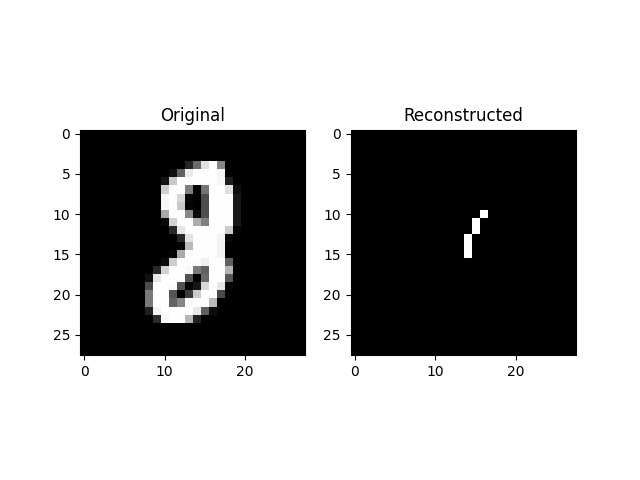
\includegraphics[width=.3\textwidth]{vae_fail.png}
    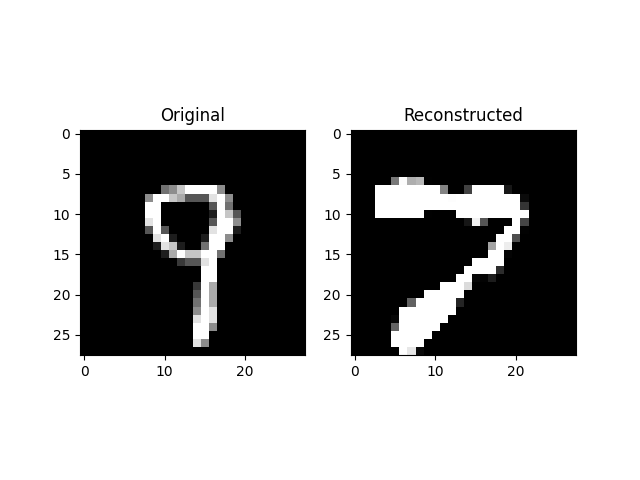
\includegraphics[width=.3\textwidth]{vae_half_fail.png}
    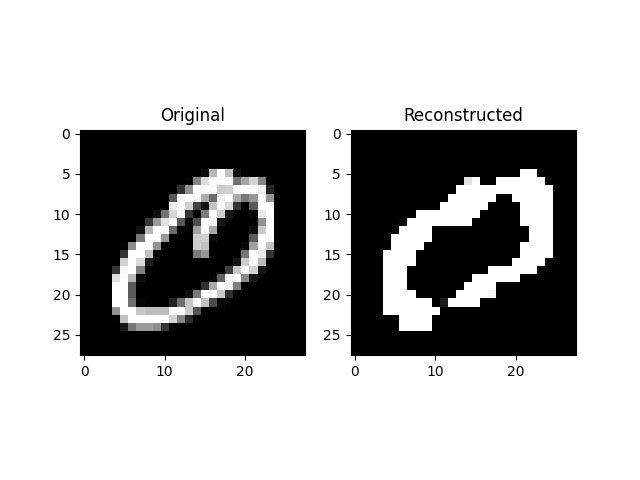
\includegraphics[width=.3\textwidth]{vae_success.png}
    \caption{Three VAE generations of increasing faithfulness to the original training data.}
    \label{fig:vae-gen}
\end{figure}

In \ref{fig:vae-gen}, we see three examples of images generated by the VAE compared to the original data points it was tasked with reconstructing. The leftmost image is an example of a degenerate output with the VAE unable to output an image resembling an 8. In the middle image, the VAE nearly produces a 9, instead generating a 7, which looks similar to a 9. During training, the VAE's latent representation of images of 7 is likely very close to those of 9. Finally, the rightmost image shows a faithful reconstruction of the training image of the number 0.
\begin{figure}
    \centering
    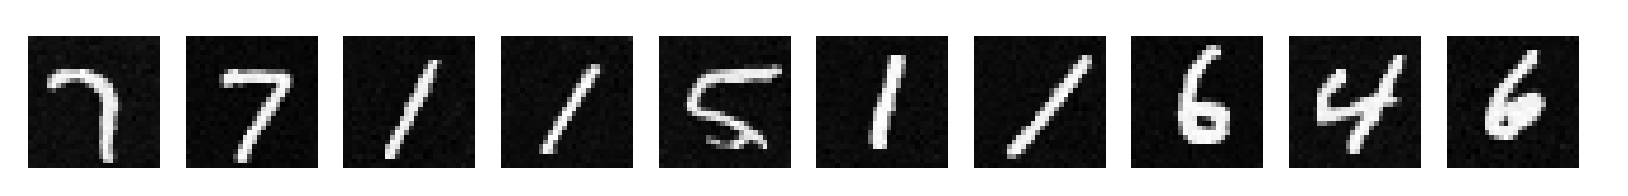
\includegraphics[scale=0.25]{ddpm_outputs_10.png}
    \caption{Ten example outputs of the DDPM.}
    \label{fig:ddpm-gen}
\end{figure}
In \ref{fig:ddpm-gen}, we observe ten example of images generated by the DDPM. Since DDPMs do not generate images from sampling from a latent code produced by encoding a given image, we are only able to assess the quality of its outputs from randomly initialized noise rather than compare them with ground-truth images. We see that the DDPM generally outputs higher-fidelity outputs than the VAE and does not produce as many degenerate images. We see that there is a general lack of diversity in the samples generated, however, although this may be mitigated by new work on reducing data bias in diffusion models. We note that DDPM took substantially longer to converge, taking over 3 hours, while the VAE took only around 45 minutes on a single machine with an Nvidia RTX 3090 GPU. While the differences in architecture are apparent, the diffusion process takes considerably longer than simply encoding an image and decoding its latent in a single step.
\section{Conclusion}
In summary, both variational autoencoders and diffusion models are latent variable models for encoding complex distributions. They both use variational inference methods to approximate intractable integrals and complex distributions more efficiently than prior approaches. To do this, both methods turn the integral into an optimization process by finding a lower bound on the data's likelihood which they can maximize directly. Both methods require reparametrization to avoid non-differentiable sampling operations in intermediate distributions.  The two methods differ in how they represent the image generation process. Variational autoencoders model the process as sampling from the latent distribution, then sampling from the data's posterior. Diffusion models similarly model the latent distribution, but over several timesteps, each with their own latent variable, and increasing fidelity, until an image from the data distribution is created (reverse process). The many transition steps potentially allow for more expressiveness in the model, which may explain why diffusion models and their variants have become the state of the art for generative image models.
\clearpage
\bibliography{report}
\bibliographystyle{abbrvnat}
\end{document}

